\documentclass{beamer}
\usefonttheme[onlymath]{serif}
\usepackage[T1]{fontenc}
\usepackage[utf8]{inputenc}
\usepackage[english]{babel}
\usepackage{amsmath}
\usepackage{amssymb}
\usepackage{amsthm}
\usepackage{gensymb}
\usepackage{parskip}
\usepackage{mathtools}
\usepackage{listings}
\usepackage{hyperref}
\usepackage{graphicx}
\usepackage{color}
\usepackage{enumerate}
\usepackage{tikz}
\usetikzlibrary{calc}
\usetikzlibrary{positioning}
\usetikzlibrary{angles}
\usetikzlibrary{shapes}
\usetikzlibrary{arrows}
\usepackage{verbatim}
\usepackage{multicol}
\usepackage{array}
\usepackage{minted}
\parskip 0pt


\DeclareMathOperator{\lcm}{lcm}
\newcommand\floor[1]{\left\lfloor#1\right\rfloor}
\newcommand\ceil[1]{\left\lceil#1\right\rceil}
\newcommand\abs[1]{\left|#1\right|}
\newcommand\p[1]{\left(#1\right)}
\newcommand\sqp[1]{\left[#1\right]}
\newcommand\cp[1]{\left\{#1\right\}}
\newcommand\norm[1]{\left\lVert#1\right\rVert}
\renewcommand\Im{\operatorname{Im}}
\renewcommand\Re{\operatorname{Re}}

\usetheme{metropolis}
\definecolor{dark yellow}{rgb} {0.6,0.6,0.0}
\definecolor{dark green}{rgb} {0.0,0.6,0.0}

\graphicspath{{myndir/}}

\title{Complexity and standard libraries}
\author{Atli FF}
\institute{\href{http://ru.is/td}{School of Computer Science} \\[2pt] \href{http://ru.is}{Reykjavík University}}
\titlegraphic{\hfill
\includegraphics[height=0.6cm]{kattis}}

\begin{document}
\maketitle


\begin{frame}[plain]{Overview for today}
    \vspace{20pt}
    \begin{itemize}
        \item Comments on inputs
        \item Basic data types
        \item Complexities
        \item Standard libraries
        \item Why we need data structures
        \item Standard library data structures
    \end{itemize}
\end{frame}

\begin{frame}[plain]{Inputs}
    \begin{itemize}
        \item As mentioned in the last lecture, when doing I/O \textbf{only print what is asked of in the output description}.
        \item Do not use \texttt{input("Please enter a number:")} or something equivalent, this prints to stdout.
        \vspace{15pt}
        \begin{tabular}{l|l|l}
            Language & Stdin & Stdout \\ \hline
            C & \texttt{scanf} & \texttt{printf} \\
            C++ & \texttt{cin} & \texttt{cout} \\
            Python & \texttt{input()} & \texttt{print()} \\
            Java & \texttt{Scanner(System.in)} & \texttt{System.out.print} \\
        \end{tabular}
    \end{itemize}
\end{frame}

\begin{frame}[plain]{Speeding up I/O}
    \begin{itemize}
        \item If fast I/O is needed, \texttt{sys.stdin} and \texttt{sys.stdout} are slightly faster in python.
        \item Similarly for fast I/O in Java, look up Kattio, it is much \textit{much} faster. It can be found on github.
        \item To speed up C++ I/O somewhat one can use \texttt{ios\_{}base::sync\_{}with\_{}stdio(false)}. Note that if this is done \texttt{scanf} or \texttt{printf} no longer sync up with \texttt{cin} and \texttt{cout}, so you have to pick one set and stick to it. Similarly \texttt{cin.tie(nullptr)} can speed things up as cout will no longer flush before cin is used, but this can cause problems when this behaviour is desired.
    \end{itemize}
\end{frame}

\section*{Basic data types}

\begin{frame}[plain]{Basic data types}
    \begin{itemize}
        \vspace{20pt}

        \item Most languages contain some version of the following:

        \begin{itemize}
            \item \texttt{bool}: a boolean (\texttt{true}/\texttt{false})
            \vspace{5pt}
            \item \texttt{char/int8\_t}: an 8-bit signed integer (often used to represent characters with ASCII)
            \item \texttt{int32\_t, int64\_t, ...}: Signed fixed size integers
            \item \texttt{uint32\_t, uint64\_t, ...}: Unsigned fixed size integers
            \vspace{5pt}
            \item \texttt{float}: an IEEE 32-bit floating-point number
            \item \texttt{double}: an IEEE 64-bit floating-point number
            \vspace{5pt}
            \item \texttt{string}: a string of characters
        \end{itemize}
    \end{itemize}
\end{frame}

\begin{frame}[plain]{Basic data types}

    {\scriptsize
        \begin{center}
            \begin{tabular}{l|lll}
                Type & Bytes & Min value & Max value \\
                \hline
                bool & 1 & & \\
                int8\_t & 1 & -128 & 127 \\
                int16\_t & 2 & -32768 & 32767 \\
                int32\_t & 4 & -2148364748 & 2147483647 \\
                int64\_t & 8 & -9223372036854775808 & 9223372036854775807 \\
                          & $n$ & $-2^{8n-1}$ & $2^{8n-1}-1$
            \end{tabular}
        \end{center}
    }

    {\scriptsize
        \begin{center}
            \begin{tabular}{l|lll}
                Type & Bytes & Min value & Max value \\
                \hline
                uint8\_t & 1 & 0 & 255 \\
                uint16\_t & 2 & 0 & 65535 \\
                uint32\_t & 4 & 0 & 4294967295 \\
                uint64\_t & 8 & 0 & 18446744073709551615 \\
                    & $n$ & $0$ & $2^{8n}-1$
            \end{tabular}
        \end{center}
    }

    {\scriptsize
        \begin{center}
            \begin{tabular}{l|llll}
                Type & Bytes & Min value & Max value & Precision \\
                \hline
                float & 4 & $\approx -3.4\times 10^{38}$ & $\approx 3.4\times 10^{38}$ & $\approx 7$ digits \\
                double & 8 & $\approx -1.7\times 10^{308}$ & $\approx 1.7\times 10^{308}$ & $\approx 14$ digits \\
            \end{tabular}
        \end{center}
    }

\end{frame}

\begin{frame}[plain]{Big integers}
    \begin{itemize}
        \item What if we need to represent and do computations with very large integers, i.e.\ something that doesn't fit in a \texttt{\_\_int128}

        \vspace{5pt}
        \item Simple idea: Store the integer as a string
        \vspace{5pt}
        \item But how do we perform arithmetic on a pair of strings?
        \item We can use the same algorithms as we learned in elementary school
            \begin{itemize}
                \item Addition: Add digit-by-digit, and maintain the carry
                \item Subtraction: Similar to addition
                \item Multiplication: Long multiplication
                \item Division: Long division
                \item Modulo: Long division
            \end{itemize}
    \end{itemize}
\end{frame}

\begin{frame}[plain]{Example problem: Simple Addition}
    \begin{itemize}
        \item https://open.kattis.com/problems/simpleaddition
        \item As can be seen on the statistics for this problem, the fastest are C/C++. But big integer operations have to be implemented manually in those languages. For these kinds of problems it can be easier to use a language that has built-in support, like Java, Python or Haskell.
    \end{itemize}
\end{frame}

\section*{Time complexities}

\begin{frame}{plain}
    \frametitle{What is a time complexity?}
    \begin{itemize}
        \item Saying a program runs in $\mathcal{O}(f(n))$ means that for some $C, n_0$ the program will take at most $C f(n)$ steps to finish for $n \geq n_0$
        \item Ignoring constants is necessary, otherwise you could change the time complexity just by making the CPU faster or adding more cores
        \item Time complexities are very useful for napkin math on whether a solution will pass time constraints
        \item For example $\mathcal{O}(n^2)$ means that as $n$ increases, the number of steps the program needs grows at most like $n^2$. So if we double $n$, the runtime might get multiplied by up to $4$
    \end{itemize}
\end{frame}

\begin{frame}{plain}
    \frametitle{Calculate time complexities}
    \begin{itemize}
        \item A good rule of thumb is that we have $10^8$ operations per second
        \only<2-> {
            \item Say we want to sort $n \leq 10^6$ integers in 3 seconds.
            \item Can we use a $\mathcal{O}(n^2)$ bubble sort or do we need to implement the more complex $\mathcal{O}(n\log(n))$ merge sort?
            \only<3-> {
                \item Bubble sort would take $\sim 10^{12}$ operations or about $10^4$ seconds, which is far too slow.
                \item The merge sort would be around $0.2$ seconds, which suffices.
            }
        }
    \end{itemize}
\end{frame}

\begin{frame}[plain]
    \frametitle{Time complexities cntd.}
    \begin{itemize}
        \item Always use the simplest solution that suffices. If $n$ had been $10^3$ bubble sort would suffice.
        \item It can be good to be able to estimate these things quick in your head.
        \item Rules of thumb can be useful, things like $2^{10} \approx 10^3$.
        \item Logarithms are usually base $2$, so like earlier if $n = 10^6$ for $n\log(n)$ we can estimate it as $10^6 \log_2(2^{20})$ or $2 \cdot 10^7$.
    \end{itemize}
\end{frame}

\begin{frame}[plain]
    \frametitle{Complexity overview}
    \scriptsize
    \begin{center}
        \begin{tabular}{c|c|c}
            $n$ & Slowest Accepted Algorithm & Example \\
            \hline
            $\leq 10$ & $O(n!)$ & Enumerating a permutation \\
            $\leq 15$ & $O(2^n\times n^2)$ & Traveling salesperson DP \\
            $\leq 20$ & $O(2^n), O(n^5)$ & Bitmask DP \\
            $\leq 50$ & $O(n^4)$ & Blossom algorithm \\
            $\leq 10^2$ & $O(n^3)$ & Floyd Warshall algorithm \\
            $\leq 10^3$ & $O(n^2)$ & Bubble/Selection/Insertion sort \\
            $\leq 10^5$ & $O(n\log_2{n})$ & Merge sort, building a Segment tree \\
            $\leq 10^6$ & $O(n)$ & Linear scans like prefix sums \\
            $> 10^8$ & $O(\log_2{n}), O(1)$ & Direct formulas or digit operations \\
        \end{tabular}
    \end{center}
\end{frame}

\section*{Standard libraries}

\begin{frame}[plain]
    \frametitle{Language features}
    \begin{itemize}
        \item Kattis allows the use of standard libraries, so get acquainted with what your language of choice has to offer.
        \item Kattis does not have other packages, like algs4 (Java) or boost (C++)
        \item C++ sorts with \texttt{sort(a.begin(), a.end())}, python has \texttt{a.sort()} and Java has \texttt{Arrays.sort(a)}.
        \item All three languages support common mathematical operations like square roots and complex numbers.
        \item C++ can do binary search with \texttt{lower\_bound} and \texttt{upper\_bound}, python can \texttt{import bisect}.
        \item There's plenty more! Regex, pseudo-randomness and plenty of data structures.
    \end{itemize}
\end{frame}

\begin{frame}[plain]
    \frametitle{Language features}
    \begin{itemize}
        \item The C++ standard library has many useful features like this
        \item \texttt{reverse} can reverse a vector or array in place
        \item \texttt{rotate} can rotate a vector or array in place
        \item \texttt{count} and \texttt{count\_if} can count elements, or count elements satisfying a predicate function
        \item \texttt{find} and \texttt{find\_if} can find an element, or find an element satisfying a predicate function
        \item And many more!
    \end{itemize}
\end{frame}

\section*{Data structures}

\begin{frame}[plain]{Why do we need data structures?}
    \begin{itemize}
        \item Sometimes our data needs to be organized in a way that allows one or more of
            \begin{itemize}
                \item Efficient querying
                \item Efficient inserting
                \item Efficient deleting
                \item Efficient updating
            \end{itemize}
        \item Sometimes we need a better way to represent our data
            \begin{itemize}
                \item How do we represent large integers?
                \item How do we represent graphs?
                \item How do we represent equivalence relations?
            \end{itemize}

        \item Data structures help us achieve those things
    \end{itemize}
\end{frame}

\begin{frame}[plain]{Data structures you should (hopefully) be familiar with}
    \begin{itemize}
    \item Static arrays \onslide<2->{- \alert{T arr[n]}}
    \item Dynamic arrays \onslide<2->{- \alert{vector<T>}}
    \item Linked lists \onslide<2->{- \alert{list<T>}}
    \item Stacks \onslide<2->{- \alert{stack<T>}}
    \item Queues \onslide<2->{- \alert{queue<T>}}
    \item Priority queues \onslide<2->{- \alert{priority\_{}queue<T>}}
    \item Ordered trees \onslide<2->{- \alert{set<T>}}
    \item Hash maps \onslide<2->{- \alert{unordered\_map<K,V>}}
    \end{itemize}
\end{frame}

\begin{frame}[plain]{Data structures in standard libraries}
    \begin{itemize}
        \item Usually it's best to use the standard library implementations
        \begin{itemize}
            \item Almost surely bug-free and fast
            \item We don't need to write any code
        \end{itemize}
        \item Sometimes we need our own implementation
        \begin{itemize}
            \item When we want more flexibility
            \item When we want to customize the data structure
        \end{itemize}
        \item And sometimes we need data structures not in the standard library, but that waits until later in the course
    \end{itemize}
\end{frame}

\begin{frame}[plain]{Applications of Arrays and Vectors}
    \begin{itemize}
        \item Too many to list
        \item Most problems require storing data, usually in an array
        \item Vectors are similar but are dynamically allocated
    \end{itemize}
    \vspace*{1cm}
    \begin{center}
    \begin{tabular}{l|l|l}
    Operation & Array complexity & Vector complexity \\ \hline
    Access element & $\mathcal{O}(1)$ & $\mathcal{O}(1)$ \\
    Append element & $\mathcal{O}(n)$ & $\mathcal{O}(1)$ \\
    Delete/insert element & $\mathcal{O}(n)$ & $\mathcal{O}(n)$ \\
    Combine arrays/vectors & $\mathcal{O}(n)$ & $\mathcal{O}(n)$ \\
    \end{tabular}
    \end{center}
\end{frame}

\begin{frame}[plain]{Applications of Linked lists}
    \begin{itemize}
        \item Very rarely used
        \item Mostly used when concatenation of arrays or insertion outside of endpoints needs to be fast
    \end{itemize}
    \vspace*{1cm}
    \begin{center}
    \begin{tabular}{l|l}
    Operation & Complexity \\ \hline
    Access element & $\mathcal{O}(n)$ \\
    Append/prepend element & $\mathcal{O}(1)$ \\
    Delete/insert at pointer & $\mathcal{O}(1)$ \\
    Combine lists & $\mathcal{O}(1)$ \\
    \end{tabular}
    \end{center}
\end{frame}

\begin{frame}[plain]{Applications of Stacks}
    \begin{itemize}
        \item Processing events in a last-in first-out order
        \item Simulating recursion
        \item Depth-first search in a graph
        \item Matching brackets
        \item And a lot more
    \end{itemize}
    \vspace*{1cm}
    \begin{center}
    \begin{tabular}{l|l}
    Operation & Complexity \\ \hline
    Push element & $\mathcal{O}(1)$ \\
    Access most recent element & $\mathcal{O}(1)$ \\
    Pop most recent element & $\mathcal{O}(1)$ \\
    \end{tabular}
    \end{center}
\end{frame}

\begin{frame}[plain]{Applications of Queues}
    \begin{itemize}
        \item Processing events in a first-in first-out order
        \item Breadth-first search in a graph
        \item And a lot more
    \end{itemize}
    \vspace*{1cm}
    \begin{center}
    \begin{tabular}{l|l}
    Operation & Complexity \\ \hline
    Push element & $\mathcal{O}(1)$ \\
    Access oldest element & $\mathcal{O}(1)$ \\
    Pop oldest element & $\mathcal{O}(1)$ \\
    \end{tabular}
    \end{center}
\end{frame}

\begin{frame}[plain]{Applications of Heaps/Priority Queues}
    \begin{itemize}
        \item Processing events in order of priority
        \item Finding a shortest path in a graph
        \item Some greedy algorithms
        \item And a lot more
    \end{itemize}
    \vspace*{1cm}
    \begin{center}
    \begin{tabular}{l|l}
    Operation & Complexity \\ \hline
    Push element & $\mathcal{O}(\log(n))$ \\
    Access highest priority element & $\mathcal{O}(1)$ \\
    Pop highest priority element & $\mathcal{O}(\log(n))$ \\
    \end{tabular}
    \end{center}
\end{frame}

\begin{frame}[plain]{Applications of Sets}
    \begin{itemize}
        \item Keep track of distinct items
        \item If implemented as a binary search tree:
        \begin{itemize}
            \item Find next greater element
            \item Count how many elements are less than a given element
            \item Find the $k$th largest element
        \end{itemize}
        \item And a lot more
    \end{itemize}
    \vspace*{1cm}
    \begin{center}
    \begin{tabular}{l|l}
    Operation & Complexity \\ \hline
    Access/check for element & $\mathcal{O}(\log(n))$ \\
    Insert/delete element & $\mathcal{O}(\log(n))$ \\
    \end{tabular}
    \end{center}
\end{frame}

\begin{frame}[plain]{Applications of Hash maps}
    \begin{itemize}
        \item Associating a value with a key
        \item As a frequency table
        \item And a lot more
    \end{itemize}
    \vspace*{1cm}
    \begin{center}
    \begin{tabular}{l|l}
    Operation & Complexity \\ \hline
    Access/check for element & $\mathcal{O}(1)$ average, $\mathcal{O}(n)$ worst case \\
    Insert/delete element & $\mathcal{O}(1)$ average, $\mathcal{O}(n)$ worst case \\
    \end{tabular}
    \end{center}
\end{frame}



\section*{Using data structures}

\begin{frame}[plain]{How to use data structures}
    \begin{itemize}
        \item In many cases you don't need fancy data structure, you just have to use simple ones in a smart way.
        \item Let us consider next the problem of NGE (Next Greater Element).
        \item We have an array of numbers. For each of the numbers we want to know where the next element to the right that is greater than it is located.
        \item Example: \texttt{[6, 2, 4, 7, 1] -> [3, 2, 3, NULL, NULL]}. Note that this is zero-indexed.
    \end{itemize}
\end{frame}

\begin{frame}[plain]{Naïve NGE}
    \begin{itemize}
        \item We could always just walk to the right for every element. 
        \only<2-> { \item But what happens for a decreasing list then? }
        \only<3-> { \item The time complexity is $\mathcal{O}(n^2)$! Far too slow. }
    \end{itemize}
\end{frame}

\begin{frame}[plain]{Smart NGE}
    \begin{itemize}
        \item Let us consider a better algorithm. Let us start with a stack $s$.
        \item We then walk through the list from left to right and add values to the stack as we go.
        \item If what we want to put on the stack is bigger than the top element, the top element must have our current element as its NGE.
        \item Thus we set that in our output and pop the top element, repeating as necessary, before putting our new element on top.
        \item At the end our output vector will contain the answer.
        \item This will then give us a $\mathcal{O}(n)$ NGE solution. Let's see an example.
    \end{itemize}
\end{frame}

\defverbatim{\ngeAA}{
\begin{verbatim}
 0 1 2 3 4 5 6 7
[2 3 1 5 7 6 4 8]
|
 0 1 2 3 4 5 6 7
[x x x x x x x x]
h: []
\end{verbatim} 
}

\defverbatim{\ngeAB}{
\begin{verbatim}
 0 1 2 3 4 5 6 7
[2 3 1 5 7 6 4 8]
 |
 0 1 2 3 4 5 6 7
[x x x x x x x x]
h: []
\end{verbatim} 
}

\defverbatim{\ngeAC}{
\begin{verbatim}
 0 1 2 3 4 5 6 7
[2 3 1 5 7 6 4 8]
 |
 0 1 2 3 4 5 6 7
[x x x x x x x x]
h: [0]
\end{verbatim} 
}

\defverbatim{\ngeAD}{
\begin{verbatim}
 0 1 2 3 4 5 6 7
[2 3 1 5 7 6 4 8]
   |
 0 1 2 3 4 5 6 7
[x x x x x x x x]
h: [0]
\end{verbatim} 
}

\defverbatim{\ngeAE}{
\begin{verbatim}
 0 1 2 3 4 5 6 7
[2 3 1 5 7 6 4 8]
 ^ |
 0 1 2 3 4 5 6 7
[x x x x x x x x]
h: [0]
\end{verbatim} 
}

\defverbatim{\ngeAF}{
\begin{verbatim}
 0 1 2 3 4 5 6 7
[2 3 1 5 7 6 4 8]
 ^ |
 0 1 2 3 4 5 6 7
[1 x x x x x x x]
h: [0]
\end{verbatim} 
}

\defverbatim{\ngeAG}{
\begin{verbatim}
 0 1 2 3 4 5 6 7
[2 3 1 5 7 6 4 8]
   |
 0 1 2 3 4 5 6 7
[1 x x x x x x x]
h: []
\end{verbatim} 
}

\defverbatim{\ngeAH}{
\begin{verbatim}
 0 1 2 3 4 5 6 7
[2 3 1 5 7 6 4 8]
   |
 0 1 2 3 4 5 6 7
[1 x x x x x x x]
h: [1]
\end{verbatim} 
}

\defverbatim{\ngeAI}{
\begin{verbatim}
 0 1 2 3 4 5 6 7
[2 3 1 5 7 6 4 8]
     |
 0 1 2 3 4 5 6 7
[1 x x x x x x x]
h: [1]
\end{verbatim} 
}

\defverbatim{\ngeAJ}{
\begin{verbatim}
 0 1 2 3 4 5 6 7
[2 3 1 5 7 6 4 8]
   ^ |
 0 1 2 3 4 5 6 7
[1 x x x x x x x]
h: [1]
\end{verbatim} 
}

\defverbatim{\ngeAK}{
\begin{verbatim}
 0 1 2 3 4 5 6 7
[2 3 1 5 7 6 4 8]
     |
 0 1 2 3 4 5 6 7
[1 x x x x x x x]
h: [1]
\end{verbatim} 
}

\defverbatim{\ngeAL}{
\begin{verbatim}
 0 1 2 3 4 5 6 7
[2 3 1 5 7 6 4 8]
     |
 0 1 2 3 4 5 6 7
[1 x x x x x x x]
h: [1 2]
\end{verbatim} 
}

\defverbatim{\ngeAM}{
\begin{verbatim}
 0 1 2 3 4 5 6 7
[2 3 1 5 7 6 4 8]
       |
 0 1 2 3 4 5 6 7
[1 x x x x x x x]
h: [1 2]
\end{verbatim} 
}

\defverbatim{\ngeAN}{
\begin{verbatim}
 0 1 2 3 4 5 6 7
[2 3 1 5 7 6 4 8]
     ^ |
 0 1 2 3 4 5 6 7
[1 x x x x x x x]
h: [1 2]
\end{verbatim} 
}

\defverbatim{\ngeAO}{
\begin{verbatim}
 0 1 2 3 4 5 6 7
[2 3 1 5 7 6 4 8]
     ^ |
 0 1 2 3 4 5 6 7
[1 x 3 x x x x x]
h: [1 2]
\end{verbatim} 
}

\defverbatim{\ngeAP}{
\begin{verbatim}
 0 1 2 3 4 5 6 7
[2 3 1 5 7 6 4 8]
   ^   |
 0 1 2 3 4 5 6 7
[1 x 3 x x x x x]
h: [1]
\end{verbatim} 
}

\defverbatim{\ngeAQ}{
\begin{verbatim}
 0 1 2 3 4 5 6 7
[2 3 1 5 7 6 4 8]
   ^   |
 0 1 2 3 4 5 6 7
[1 3 3 x x x x x]
h: [1]
\end{verbatim} 
}

\defverbatim{\ngeAR}{
\begin{verbatim}
 0 1 2 3 4 5 6 7
[2 3 1 5 7 6 4 8]
       |
 0 1 2 3 4 5 6 7
[1 3 3 x x x x x]
h: []
\end{verbatim} 
}

\defverbatim{\ngeAS}{
\begin{verbatim}
 0 1 2 3 4 5 6 7
[2 3 1 5 7 6 4 8]
       |
 0 1 2 3 4 5 6 7
[1 3 3 x x x x x]
h: [3]
\end{verbatim} 
}

\defverbatim{\ngeAT}{
\begin{verbatim}
 0 1 2 3 4 5 6 7
[2 3 1 5 7 6 4 8]
         |
 0 1 2 3 4 5 6 7
[1 3 3 x x x x x]
h: [3]
\end{verbatim} 
}

\defverbatim{\ngeAU}{
\begin{verbatim}
 0 1 2 3 4 5 6 7
[2 3 1 5 7 6 4 8]
       ^ |
 0 1 2 3 4 5 6 7
[1 3 3 x x x x x]
h: [3]
\end{verbatim} 
}

\defverbatim{\ngeAV}{
\begin{verbatim}
 0 1 2 3 4 5 6 7
[2 3 1 5 7 6 4 8]
       ^ |
 0 1 2 3 4 5 6 7
[1 3 3 4 x x x x]
h: [3]
\end{verbatim} 
}

\defverbatim{\ngeAW}{
\begin{verbatim}
 0 1 2 3 4 5 6 7
[2 3 1 5 7 6 4 8]
         |
 0 1 2 3 4 5 6 7
[1 3 3 4 x x x x]
h: []
\end{verbatim} 
}

\defverbatim{\ngeAX}{
\begin{verbatim}
 0 1 2 3 4 5 6 7
[2 3 1 5 7 6 4 8]
         |
 0 1 2 3 4 5 6 7
[1 3 3 4 x x x x]
h: [4]
\end{verbatim} 
}

\defverbatim{\ngeAY}{
\begin{verbatim}
 0 1 2 3 4 5 6 7
[2 3 1 5 7 6 4 8]
           |
 0 1 2 3 4 5 6 7
[1 3 3 4 x x x x]
h: [4]
\end{verbatim} 
}

\defverbatim{\ngeAZ}{
\begin{verbatim}
 0 1 2 3 4 5 6 7
[2 3 1 5 7 6 4 8]
         ^ |
 0 1 2 3 4 5 6 7
[1 3 3 4 x x x x]
h: [4]
\end{verbatim} 
}

\defverbatim{\ngeBA}{
\begin{verbatim}
 0 1 2 3 4 5 6 7
[2 3 1 5 7 6 4 8]
           |
 0 1 2 3 4 5 6 7
[1 3 3 4 x x x x]
h: [4]
\end{verbatim} 
}

\defverbatim{\ngeBB}{
\begin{verbatim}
 0 1 2 3 4 5 6 7
[2 3 1 5 7 6 4 8]
           |
 0 1 2 3 4 5 6 7
[1 3 3 4 x x x x]
h: [4 5]
\end{verbatim} 
}

\defverbatim{\ngeBC}{
\begin{verbatim}
 0 1 2 3 4 5 6 7
[2 3 1 5 7 6 4 8]
             |
 0 1 2 3 4 5 6 7
[1 3 3 4 x x x x]
h: [4 5]
\end{verbatim} 
}

\defverbatim{\ngeBD}{
\begin{verbatim}
 0 1 2 3 4 5 6 7
[2 3 1 5 7 6 4 8]
           ^ |
 0 1 2 3 4 5 6 7
[1 3 3 4 x x x x]
h: [4 5]
\end{verbatim} 
}

\defverbatim{\ngeBE}{
\begin{verbatim}
 0 1 2 3 4 5 6 7
[2 3 1 5 7 6 4 8]
             |
 0 1 2 3 4 5 6 7
[1 3 3 4 x x x x]
h: [4 5]
\end{verbatim} 
}

\defverbatim{\ngeBF}{
\begin{verbatim}
 0 1 2 3 4 5 6 7
[2 3 1 5 7 6 4 8]
             |
 0 1 2 3 4 5 6 7
[1 3 3 4 x x x x]
h: [4 5 6]
\end{verbatim} 
}

\defverbatim{\ngeBG}{
\begin{verbatim}
 0 1 2 3 4 5 6 7
[2 3 1 5 7 6 4 8]
               |
 0 1 2 3 4 5 6 7
[1 3 3 4 x x x x]
h: [4 5 6]
\end{verbatim} 
}

\defverbatim{\ngeBH}{
\begin{verbatim}
 0 1 2 3 4 5 6 7
[2 3 1 5 7 6 4 8]
             ^ |
 0 1 2 3 4 5 6 7
[1 3 3 4 x x x x]
h: [4 5 6]
\end{verbatim} 
}

\defverbatim{\ngeBI}{
\begin{verbatim}
 0 1 2 3 4 5 6 7
[2 3 1 5 7 6 4 8]
             ^ |
 0 1 2 3 4 5 6 7
[1 3 3 4 x x 7 x]
h: [4 5 6]
\end{verbatim} 
}

\defverbatim{\ngeBJ}{
\begin{verbatim}
 0 1 2 3 4 5 6 7
[2 3 1 5 7 6 4 8]
           ^   |
 0 1 2 3 4 5 6 7
[1 3 3 4 x x 7 x]
h: [4 5]
\end{verbatim} 
}

\defverbatim{\ngeBK}{
\begin{verbatim}
 0 1 2 3 4 5 6 7
[2 3 1 5 7 6 4 8]
           ^   |
 0 1 2 3 4 5 6 7
[1 3 3 4 x 7 7 x]
h: [4 5]
\end{verbatim} 
}

\defverbatim{\ngeBL}{
\begin{verbatim}
 0 1 2 3 4 5 6 7
[2 3 1 5 7 6 4 8]
         ^     |
 0 1 2 3 4 5 6 7
[1 3 3 4 x 7 7 x]
h: [4]
\end{verbatim} 
}

\defverbatim{\ngeBM}{
\begin{verbatim}
 0 1 2 3 4 5 6 7
[2 3 1 5 7 6 4 8]
         ^     |
 0 1 2 3 4 5 6 7
[1 3 3 4 7 7 7 x]
h: [4]
\end{verbatim} 
}

\defverbatim{\ngeBN}{
\begin{verbatim}
 0 1 2 3 4 5 6 7
[2 3 1 5 7 6 4 8]
               |
 0 1 2 3 4 5 6 7
[1 3 3 4 7 7 7 x]
h: []
\end{verbatim} 
}

\defverbatim{\ngeBO}{
\begin{verbatim}
 0 1 2 3 4 5 6 7
[2 3 1 5 7 6 4 8]
               |
 0 1 2 3 4 5 6 7
[1 3 3 4 7 7 7 x]
h: [8]
\end{verbatim} 
}

\defverbatim{\ngeBP}{
\begin{verbatim}
 0 1 2 3 4 5 6 7
[2 3 1 5 7 6 4 8]
 0 1 2 3 4 5 6 7
[1 3 3 4 7 7 7 x]
h: [8]
\end{verbatim} 
}

\begin{frame}[plain,fragile]
	\only<all:1>{\ngeAA}
	\only<all:2>{\ngeAB}
	\only<all:3>{\ngeAC}
	\only<all:4>{\ngeAD}
	\only<all:5>{\ngeAE}
	\only<all:6>{\ngeAF}
	\only<all:7>{\ngeAG}
	\only<all:8>{\ngeAH}
	\only<all:9>{\ngeAI}
	\only<all:10>{\ngeAJ}
	\only<all:11>{\ngeAK}
	\only<all:12>{\ngeAL}
	\only<all:13>{\ngeAM}
	\only<all:14>{\ngeAN}
	\only<all:15>{\ngeAO}
	\only<all:16>{\ngeAP}
	\only<all:17>{\ngeAQ}
	\only<all:18>{\ngeAR}
	\only<all:19>{\ngeAS}
	\only<all:20>{\ngeAT}
	\only<all:21>{\ngeAU}
	\only<all:22>{\ngeAV}
	\only<all:23>{\ngeAW}
	\only<all:24>{\ngeAX}
	\only<all:25>{\ngeAY}
	\only<all:26>{\ngeAZ}
	\only<all:27>{\ngeBA}
	\only<all:28>{\ngeBB}
	\only<all:29>{\ngeBC}
	\only<all:30>{\ngeBD}
	\only<all:31>{\ngeBE}
	\only<all:32>{\ngeBF}
	\only<all:33>{\ngeBG}
	\only<all:34>{\ngeBH}
	\only<all:35>{\ngeBI}
	\only<all:36>{\ngeBJ}
	\only<all:37>{\ngeBK}
	\only<all:38>{\ngeBL}
	\only<all:39>{\ngeBM}
	\only<all:40>{\ngeBN}
	\only<all:41>{\ngeBO}
	\only<all:42>{\ngeBP}
\end{frame}

\begin{frame}[plain,fragile]{C++ NGE}
    \begin{minted}{cpp}
template<typename T>
vector<size_t> nge(vector<T>& v) {
  vector<size_t> res(v.size(), -1);
  stack<pair<size_t,T>> s; 
  s.push(make_pair(0,v[0]));
  for(size_t i = 0; i < v.size(); ++i) {
    while(!s.empty() && s.top().second <= v[i]) {
      res[s.top().first] = i; 
      s.pop(); 
    }
    s.push(make_pair(i, v[i])); 
  }
  return res; 
}
    \end{minted}
\end{frame}


\begin{frame}[plain]{Augmenting Data Structures}
    \begin{itemize}
        \item Sometimes we can store extra information in our data structures to gain more functionality
        \item Usually we can't do this to data structures in the standard library (but there are exceptions, gnu\_pbds)
        \item Need our own implementation that we can customize
        \item Sometimes this functionality is simply better time complexity
    \end{itemize}
\end{frame}

\begin{frame}[plain]{Heaps}
    \begin{itemize}
        \item As an example of a data structure in the standard library but that sometimes requires a more powerful version, let us consider heaps.
        \item Heaps are implemented in most standard libraries in the forms of priority queues.
        \item A heap is nothing but a binary tree satisfying \textit{the heap condition}.
        \item The heap condition (for a min heap) says that the value of any given node is not greater than that of its chilren.
    \end{itemize}
\end{frame}

\begin{frame}[plain]{Heaps}
    \begin{itemize}
        \item Since arrays are linear, we want to smush this binary tree into an array for the implementation.
        \item We can do this by putting the root at index $1$. Then the children of item at index $i$ are simply at $2i$ and $2i+1$. The parent of any item $i > 1$ is then $\floor{i/2}$.
        \item We could do this using raw arrays (then index $0$ can be used to store its size), but the examples will be given in C++ using vectors.
    \end{itemize}
\end{frame}

\begin{frame}[plain]{Heaps}
    \begin{center}
    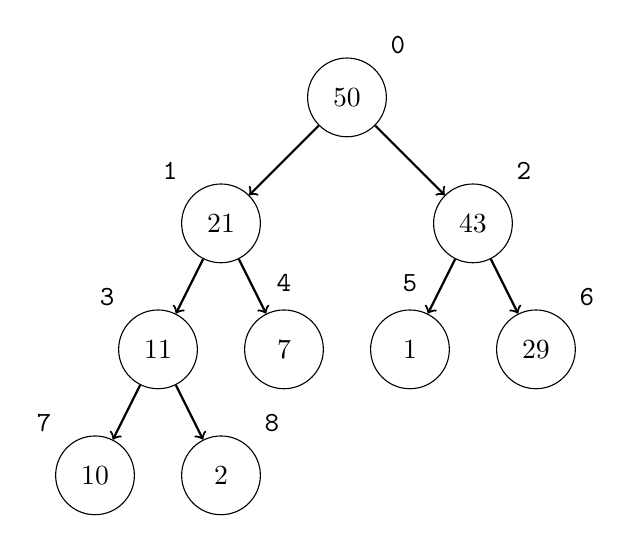
\begin{tikzpicture}[scale=0.8]
    \def\spa{2}
    \node[minimum size=1cm, draw, circle] (A) at (0, 0) {$50$};
    \node[minimum size=1cm, draw, circle] (B) at (-\spa, -\spa) {$21$};
    \node[minimum size=1cm, draw, circle] (C) at (\spa, -\spa) {$43$};
    \node[minimum size=1cm, draw, circle] (D) at (-1.5*\spa, -2*\spa) {$11$};
    \node[minimum size=1cm, draw, circle] (E) at (-0.5*\spa, -2*\spa) {$7$};
    \node[minimum size=1cm, draw, circle] (F) at (0.5*\spa, -2*\spa) {$1$};
    \node[minimum size=1cm, draw, circle] (G) at (1.5*\spa, -2*\spa) {$29$};
    \node[minimum size=1cm, draw, circle] (H) at (-2*\spa, -3*\spa) {$10$};
    \node[minimum size=1cm, draw, circle] (I) at (-\spa, -3*\spa) {$2$};
    
    \node (Ai) [above right=0.1cm of A] {\texttt{0}};
    \node (Bi) [above left=0.1cm of B] {\texttt{1}};
    \node (Ci) [above right=0.1cm of C] {\texttt{2}};
    \node (Di) [above left=0.1cm of D] {\texttt{3}};
    \node (Ei) [above=0.1cm of E] {\texttt{4}};
    \node (Fi) [above=0.1cm of F] {\texttt{5}};
    \node (Gi) [above right=0.1cm of G] {\texttt{6}};
    \node (Hi) [above left=0.1cm of H] {\texttt{7}};
    \node (Ii) [above right=0.1cm of I] {\texttt{8}};
    
    \draw[->, thick] (A) -- (B);
    \draw[->, thick] (A) -- (C);
    \draw[->, thick] (B) -- (D);
    \draw[->, thick] (B) -- (E);
    \draw[->, thick] (C) -- (F);
    \draw[->, thick] (C) -- (G);
    \draw[->, thick] (D) -- (H);
    \draw[->, thick] (D) -- (I);
    \end{tikzpicture}
    \end{center}
    \begin{large}
    \texttt{ARRAY: [SIZE, 50, 21, 43, 11, 7, 1, 29, 10, 2]}
    \end{large}
\end{frame}

\begin{frame}[plain]{Heaps}
    \begin{itemize}
        \item Items can be inserted by pushing them to the back and fixing the heap condition upwards from them.
        \item Items can be deleted by replacing the smallest value with a leaf and then fixing the heap condition downwards.
        \item Let us see how this would look in C++.
    \end{itemize}
\end{frame}

\begin{frame}[plain, fragile]{C++ implementation}
    \scriptsize
    \begin{minted}{cpp}
template<typename T> struct Heap {
    vector<T> h; Heap() : h(1) { }
    size_t size() { return h.size() - 1; }
    T peek() { return h[1]; }
    void swim(size_t i) {
        while(i != 1 && h[i] < h[i / 2]) {
            swap(h[i], h[i / 2]);
            i /= 2; } }
    void sink(size_t i) {
        while(true) {
            size_t mn = i;
            if(2 * i + 1 < h.size() && h[mn] > h[2 * i + 1]) mn = 2 * i + 1;
            if(2 * i  < h.size() && h[mn] > h[2 * i]) mn = 2 * i;
            if(mn != i) swap(h[i], h[mn]), i = mn;
            else break; } }
    void pop() {
        h[1] = h.back();
        h.pop_back(); sink(1); }
    void push(T x) {
        h.push_back(x);
        swim(h.size() - 1); } };
    \end{minted}
\end{frame}

\begin{frame}[plain]{Heaps}
    \begin{itemize}
        \item We note that peek and size run in $\mathcal{O}(1)$ while all other operations run in $\mathcal{O}(log(n))$.
        \item This can be used to, for example, solve the Bastard's Peace problem listed earlier.
        \item This implementation isn't any better than the standard library one in C++.
        \item But let us consider a harder problem where the standard heap (and this one) aren't good enough.
        \item This particular implementation won't be needed for problems in the course, it is merely an example.
    \end{itemize}
\end{frame}

\begin{frame}[plain]{Hard heap problem (Trade Routes on Kattis)}
    \begin{itemize}
        \item You are given a tree on $n \leq 300\,000$ vertices.
        \item Each of the nodes want to trade with Rome, located at node $1$. A trade route from that node puts strain on all nodes on the way from that node to Rome.
        \item Each node has a trade value which is how much would be gained from it trading with Rome.
        \item Each node has a capacity which is the maximum strain it can tolerate from trade routes.
        \item How much trade value can be gained at most?
    \end{itemize}
\end{frame}

\begin{frame}[plain]{How to use heaps}
    \begin{itemize}
        \item Imagine each node has a heap.
        \item At the start each heap just contains the trade value at that node.
        \item Then we move from the leaves inwards, merging together the heaps from children to parents as we go.
        \item This may make the heap larger than the capacity at some point, so we pop values from it until this is fixed.
        \item This would make the final heap at Rome contain the trade routes we want.
    \end{itemize}
\end{frame}

\begin{frame}[plain]{How to use heaps (?)}
    \begin{itemize}
        \item There is just one problem.
        \item The STL (standard library) implementation has a merging operation that runs in $\mathcal{O}(n)$, so this algorithm would be $\mathcal{O}(n^2)$ which is far too slow ($\sim 15$ minute runtime).
        \item Can we make our own heap that merges in $\mathcal{O}(\log(n))$ or better?
        \only<2-> { \item The reason the problem is so hard is that this implementation is rather involved. I'll put it here for completeness's sake, but we will not delve much deeper here. }
    \end{itemize}
\end{frame}

\begin{frame}[fragile, plain]{Pairing heap C++}
    \tiny
    \begin{multicols}{2}
    \begin{minted}{cpp}
struct HeapNode {
    int32_t k, v; HeapNode *lch, *sib;
    HeapNode() : lch(NULL), sib(NULL) { }
    HeapNode(int32_t _k, int32_t _v, HeapNode *_lch, 
        HeapNode *_sib) :
        k(_k), v(_v), lch(_lch), sib(_sib) { }
    void add_child(HeapNode *node) {
        if(lch == NULL) lch = node;
        else {
            node->sib = lch;
            lch = node;
        }
    }
};
struct PairingHeap {
    HeapNode* root; size_t sz;
    PairingHeap() : root(NULL), sz(0) { }
    HeapNode* merge(HeapNode* A, HeapNode* B) {
        if(A == NULL) return B;
        if(B == NULL) return A;
        if(A->k < B->k) {
            A->add_child(B);
            return A;
        }
        B->add_child(A);
        return B;
    }
    \end{minted}
    \columnbreak
    \begin{minted}{cpp}
    HeapNode* twopass(HeapNode *node) {
        if(node == NULL || node->sib == NULL) 
            return node;
        HeapNode *A = node, *B = node->sib, 
            *nw = node->sib->sib;
        A->sib = NULL; B->sib = NULL;
        return merge(merge(A, B), twopass(nw));
    }
    pair<int32_t,int32_t> top() {
        return make_pair(root->k, root->v);
    }
    void insert(int32_t k, int32_t v) {
        root = merge(root, 
            new HeapNode(k, v, NULL, NULL));
        sz++;
    }
    void pop() {
        root = twopass(root->lch);
        sz--;
    }
    void join(PairingHeap oth) {
        root = merge(root, oth.root);
        sz += oth.sz;
    }
};
    \end{minted}
    \end{multicols}
\end{frame}

\begin{frame}[plain]{How to use (fancy) heaps}
    \begin{itemize}
        \item This heap can also be used wherever you'd use the STL one as well.
        \item This one can peek, insert and merge in $\mathcal{O}(1)$ and pop in $\mathcal{O}(\log(n))$.
        \item It has more overhead though, so in practice it will be a fair bit slower than the STL one for non-merge operations.
    \end{itemize}
\end{frame}


\end{document}

